%
\chapter{Simulation of capacitively coupled rf discharges}\label{sec:chapter_twodccrf}
%
	\section{Experimental setup}\label{sec:twod_setup}
%
		Giving the necessary background in~\autoref{sec:surfaceeffects} and providing the crucially important comparison of the previous~\autoref{sec:chapter_onedcomparison}, the afore-mentioned effects of highly energetic negative oxygen ions can now be further investigated.
%
		\subsection{Reference Discharge}\label{sec:reference_dis}
%
			\begin{figure}[b!]
				\centering
				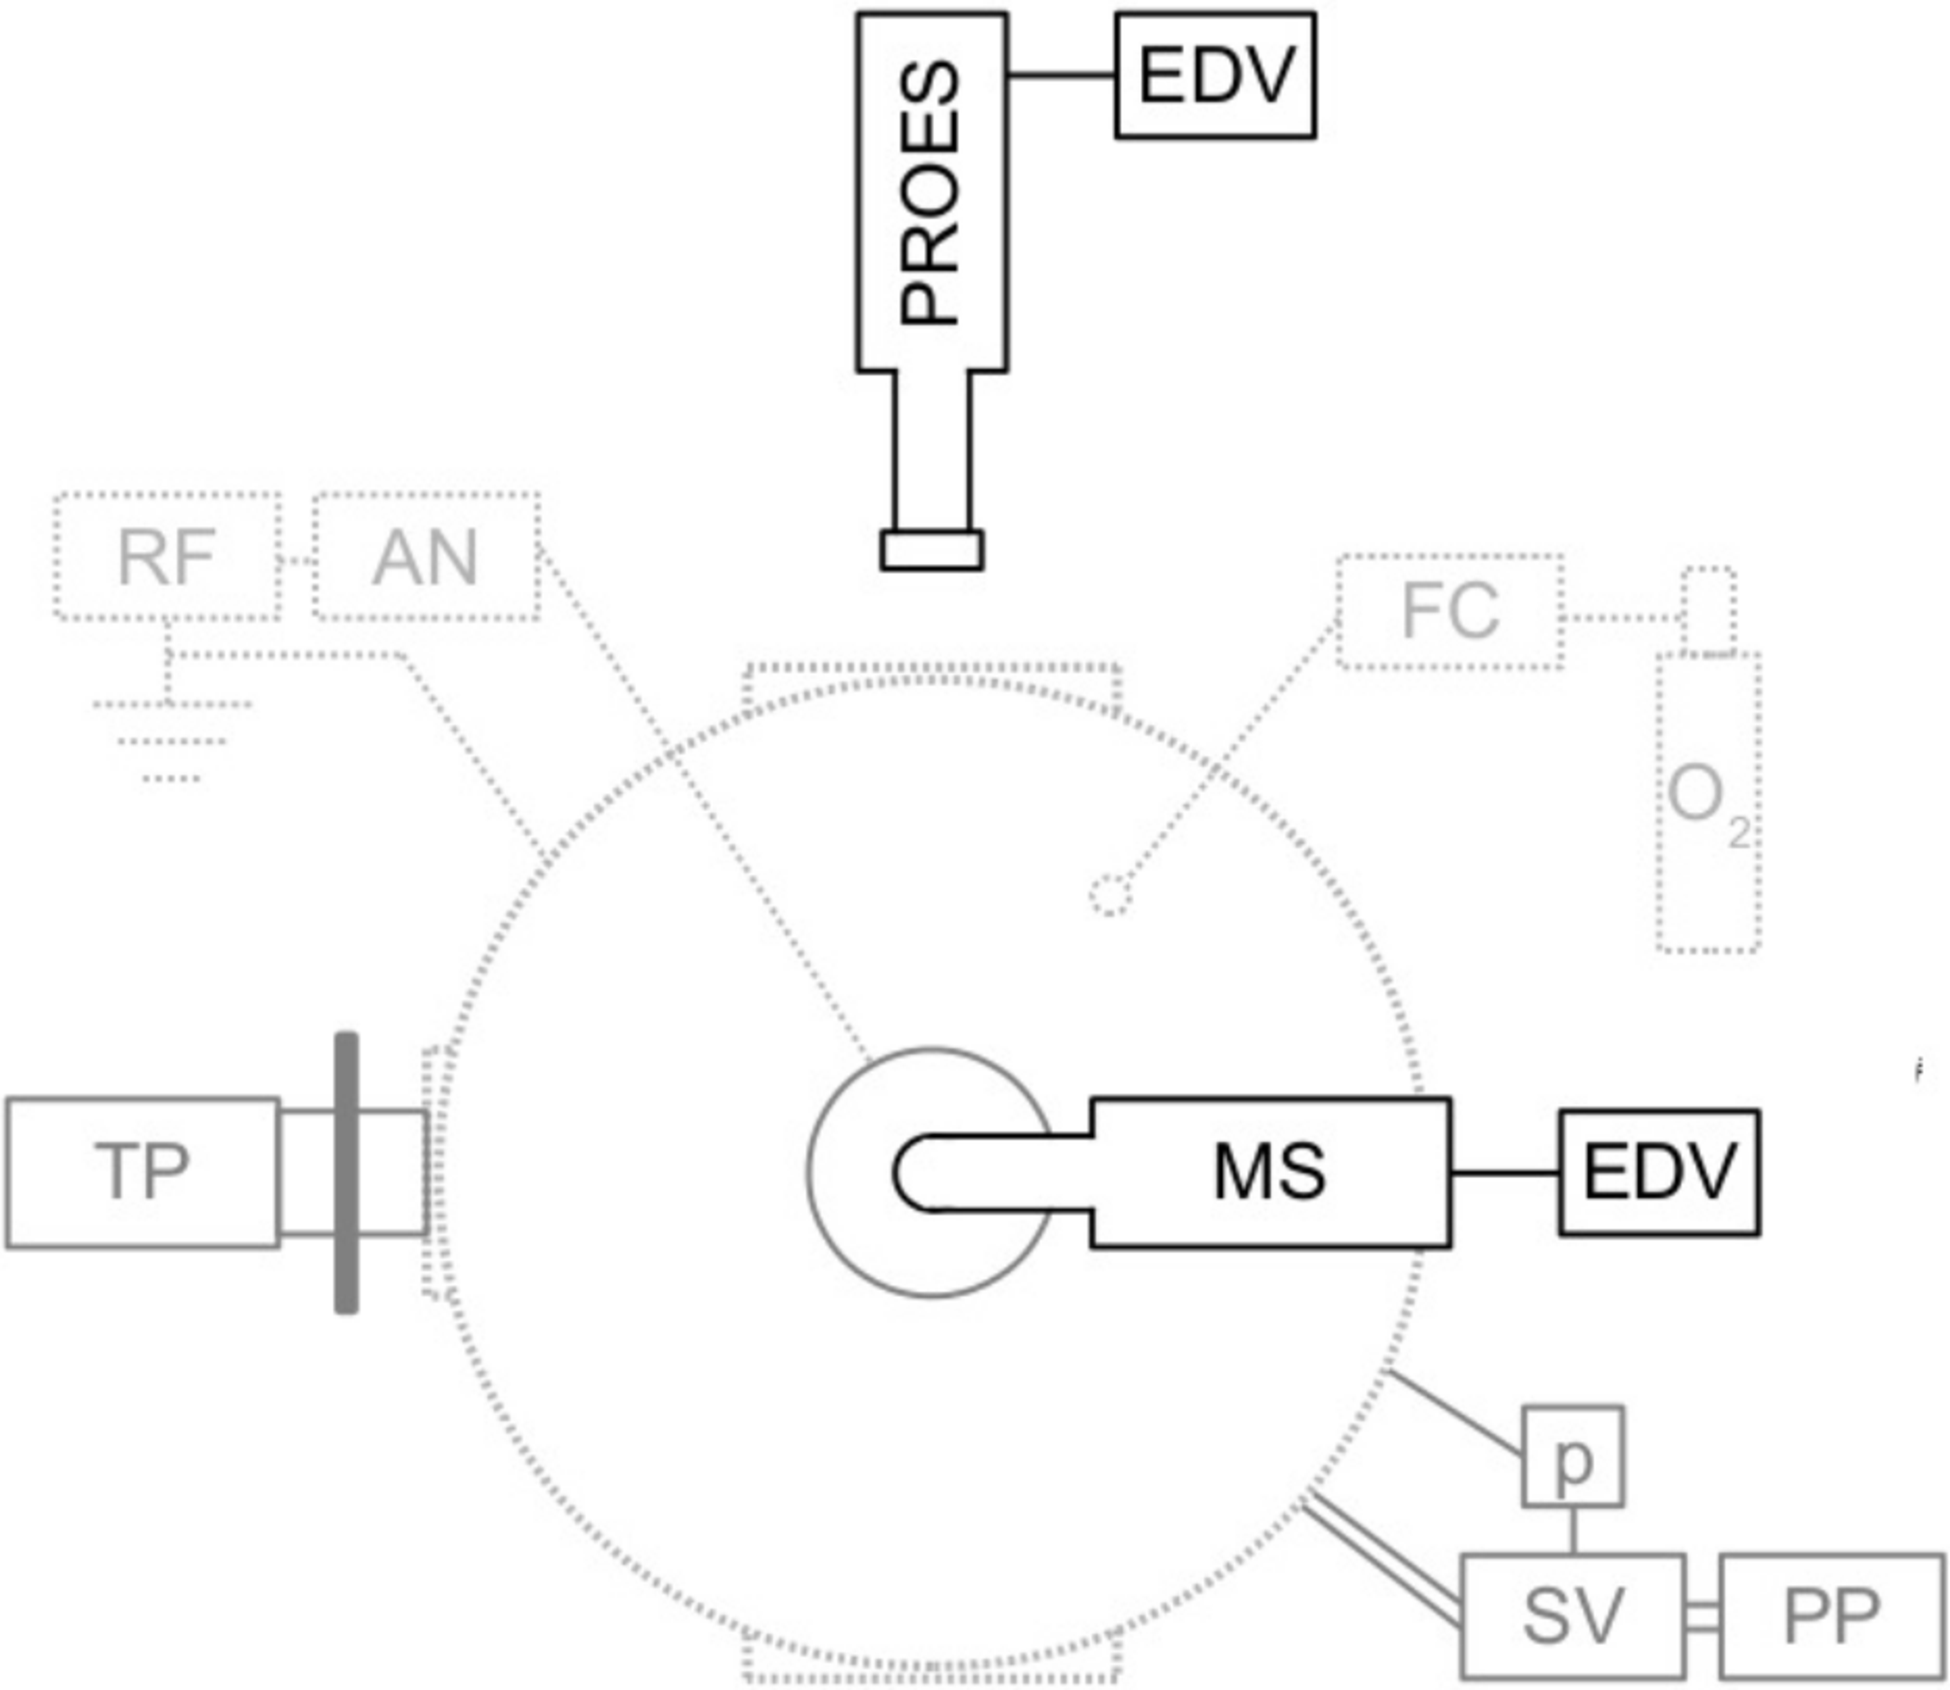
\includegraphics[width=0.5\textwidth]{figures/chamber_exp.pdf}
				\caption{%
				Top-down view schematic of the experiment~\cite{Scheuer15},~\cite{Kullig12}. Shown is the setup without microwave interferometer, like it was used by Küllig et al.}%
				\label{fig:discharge_chamber}
			\end{figure}
%
			Here, the referenced experiment was used by Küllig et al.~\cite{Kullig12} and Scheuer~\cite{Scheuer15}, and consists of a cylindrical setup, filled with oxygen at low pressures and gas flow rates (see~\autoref{fig:discharge_chamber}). The stainless steel vacuum chamber had a diameter and height of $\unit[40]{cm}$ respectively and was filled with the process gas oxygen (O$\ix{2}$) at $\unit[5]{sccm}$ (\fett{FC}). The discharge configuration consisted of an electrode in the center with $\unit[10]{cm}$ of diameter and a rf generator, constantly operating at a frequency of $\unit[13,56]{MHz}$ and power outputs between $5$ and $\unit[150]{W}$ (\fett{RF} and \fett{AN}), leading to applied voltages in the range of $100$--$\unit[1500]{V}$. Shielding and discharge enclosure/chamber walls were grounded, therefore yielding a large area ratio between driven and grounded electrode and establishing a heavily asymmetric plasma. In addition, the powered electrode was coupled capacitively with the external generator, emphasizing the effect of the, in~\autoref{sec:selfbias} introduced self bias voltage. The value of $U\ix{sb}$ ranged, depending on power output and discharge pressure, from $-100$ up to $\unit[500]{V}$. In~\cite{Kullig12} the experiment was pulsed with short discharges at a frequency of $\unit[10]{Hz}$.	Line integrated measurements resulted in an average electron density of around $\tenpo{11}$--$\unit[\tenpo{12}]{cm^{-3}}$. Showing a schematic top-down view of the experiment is~\autoref{fig:discharge_chamber}. Here, the large ratio between driven and grounded parts is very well visualized. Hence, in later simulations it will be of sufficient accuracy to restrain the virtualized volume to a smaller setup.\\
			The figure below includes further diagnostics like a mass spectrometer (\fett{MS}) and phase resolved optical emission spectroscopy (\fett{PROES}). The latter measured the mentioned densities via line integration across the plasma volume. The MS is a key instrument for the investigation pursued in this thesis, as it also measures species counts with respect to their contribution to their correspoding energy distribution function. For example, the ions created via secondary processes in the discharge sheath are accelerated towards the bulk and thus get into the MS with their characteristic speeds and mass. A significant increase of electron density was found for rf powers larger than $\unit[50]{W}$ or $\unit[-220]{V}$ self bias voltage~\cite{Kullig12}. This led to a correlating negativ oxygen ion density reduction and decrease of the electronegativity ratio $\overline{n}_{i,-}/\overline{n}\ix{e}$ from $4$ to $0,03$. During a different operation mode --- called $\alpha$-mode, contrary to the afore-mentioned $\gamma$-mode --- at less than $\unit[50]{V}$ output power, electronegativity rises again, as well as the electron temperature $T\ix{e}$, yielding higher rate coefficients for, e.g.\@ dissociative electron attachment and the alike. See~\autoref{sec:anionproduction} for a more detailed approach.
%
		\subsection{Simulated Discharge}\label{sec:simulatedd_dis}
%
			All of the above conditions are sufficient for a practical approach at a labratory ccrf discharge with great repeatability. Though being highly optimized and developed over the course of many years, the twodimensional particle-in-cell code outlined above does not provide the tools and performance to feasibly simulate such large areas and particle numbers. Hence, one will reside to reducing the numerical expense by virtualizing smaller discharge areas and average densities, while trying to satisfy the same physical processes exhibited in~\cite{Kullig12}.\\
			The afore-mentioned 2d3v PIC code is used to simulated the referenced experiment. The spatial dimensions will be the radial component $r$ and axial coordinate $z$. The geometry and simulation is optimized for cylindrically symmetric gas discharges.\\
			To represent the strong asymmetry between driven and grounded wall areas, the sizes of anode, cathode and grounded chamber parts have been chosing accordingly. The experimental values for the self bias voltage $U\ix{sb}$ were used to create a dc offset on-top of the rf voltage $U\ix{rf}$ at the cathode. The domain composition with cells of width $\lambda\ix{D,e}/2$ (see~\autoref{sec:picbasics}) makes it even more difficult to appropriately model the system. Hence a smaller discharge volume of a $\unit[4,5]{cm}$ radius and an electrode gap of $\unit[2,5]{cm}$ will be simulated. This usually leads to cell counts up to $2\cdot\tenpo{5}$, which is small in comparison to the `real' experiment, which would have to be covered by over $\tenpo{6}$ cells. Furthermore, the numerical expense grows with $N\log(N)$, and $N$ being the particle number inside the cells (see~\autoref{sec:picsimulationmcc}).\\
			One has chosen pressures between $\unit[2]{Pa}$ and $\unit[10]{Pa}$, with the possibility of changing it later during the discharges simulation --- e.g\@ to change the bulk volume and densities. The secondary ion emission efficiency was set to $\eta=0,03$ in all cases, yielding a stable plasma sheath and hence SIE current into the bulk. In addition, a constant self bias of $\unit[-200]{V}$ was appplied at the cathode. The radio frequency was set to $\unit[13,56]{MHz}$.\\
			The governing electron density and temperature were set to $\unit[5\cdot\tenpo{9}]{cm^{-3}}$ and $\unit[5]{eV}$ respectively, which, as an initial value and property for scale, is sufficient for the necessary rate coefficients mentioned above. This led to the following important scales of simulation: 
%
			\begin{align}
				\lambda\ix{D}&=\unit[0,0235]{cm}\,,%
				\hspace*{2.0cm}%
				\omega\ix{p,e}=\unit[3,99\cdot\tenpo{9}]{Hz}%
				\label{equ:debyeandomega}\\[0.0cm]
				\Rightarrow \Delta x&=\frac{1}{2}\,\lambda\ix{D}=\unit[0,01174]{cm}\,,%
				\quad\quad%
				\Delta t=0,2\cdot\omega\ix{p,e}=\unit[5,015\cdot\tenpo{-11}]{s}%
				\label{equ:simulationscales}
			\end{align}
%			
			Thus a single rf cycle at the given frequency takes $1470$ steps, and the domain measures $384$ and $213$ in radial and axial dimension respectively. An ion temperature is adjusted via the fraction $T\ix{i}/T\ix{e}=0,008$, hence the corresponding velocities for the previously defined electron temperature $T\ix{e}=\unit[5]{eV}=\unit[5,8\cdot\tenpo{4}]{K}$ are found to be
%
			\begin{align}
				v\ix{th,e}=&\,\unit[9,37\cdot\tenpo{5}]{\frac{m}{s}}\,,%
				\quad\quad%
				c\ix{s,e}=\,\unit[3,87\cdot\tenpo{3}]{\frac{m}{s}}%
				\label{equ:electronvelocities}\\[0.0cm]%
%				IONS 
				v\ix{th,i}=&\,\unit[558,38]{\frac{m}{s}}\,,%
				\hspace*{1.2cm}%
				c\ix{s,i}=\,\unit[371,44]{\frac{m}{s}}%
				\label{equ:ionvelocities}
			\end{align}
%
		\begin{wrapfigure}{r}{0.3\textwidth}
			\centering
			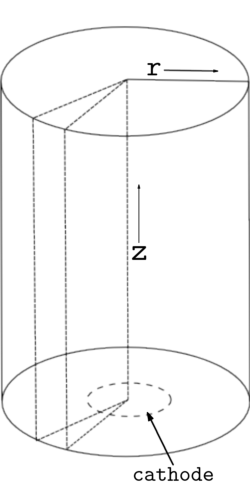
\includegraphics[width=0.275\textwidth]{figures/radial_cylinder.pdf}\\
			\vspace*{0.3cm}\hspace*{0.1cm}
			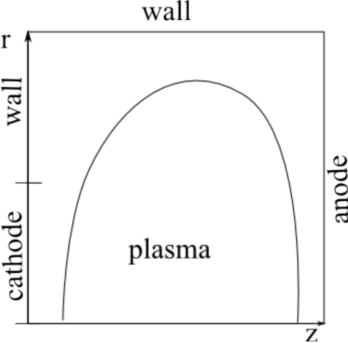
\includegraphics[width=0.275\textwidth]{figures/domain_slice.pdf}
			\caption{%
			Simplified cylinder schematic for the simulated experiment. The slice depicte in the top is shown below. There, boundaries and bulk position are outlined.}\label{fig:radialcylinder}
		\end{wrapfigure}
%
			Here, a single millisecond of operation takes days, if not weeks to simulate with a given timestep, like in~\autoref{equ:simulationscales}. Due to this and the fact, that the unit cell volume increases with the layer index of the radial coordinate --- one has to keep in mind that the cylindrical geometry is key to the simulation because important simplifications and assumptions inside the code itself are made uppon that premise ---, each particle carries an additional statistical weight. For example, a virtual neutral gas molecule of O$\ix{2}$ may represents up to $\tenpo{8}$ `real' particles in a laboratory plasma. This saves a vast amount of computational time by immensely reducing the particle counts necessary to sufficiently model the investigated physical processes. In this case, a single neutral gas particle is statistically amplified by a factor of $\approx 9,3\cdot\tenpo{7}$ to account for the gas density at $\unit[5]{Pa}$ and $\approx\unit[300]{K}$. This number is crucial to all collisional processes, where the molecular species O$\ix{2}$ is involved. Charged particle species share a common number amplification of $8489$. On top of both super particle factors, a scaling $\sim 1/r$ is applied to consider the variable cell volume.\\
			Another numerical tool is a constant neutral gas background. In the afore-metioned experiment, a working gas reservoir and flow rate meter control the pressure and exchange of O$\ix{2}$ inside the chamber. Due to the slow transition velocities of the cold neutral species, a working gas current from e.g.\@ behind an electrode is not feasible in this simulation. Collision rates and reaction coefficients are destroying neutral gas particles faster than they can be sufficiently supplied to the discharge. Hence, the O$\ix{2}$ molecules are initiated at time $t=0$ of the simulation --- this is done with respect to pressure, super particle factor and the alike ---, and are afterwards not altered in number or location. Though collision routines are still exercised, the corresponding push of the neutral species is skipped.
%
	\section{Simulated ccrf Oxygen Discharge}\label{sec:twod_secondaryions}
%
	In the collection of~\autoref{fig:2d-collection} twodimensional densities and potential are shown. Again, parameters were chosen as $U\ix{rf}=\unit[400]{V}$, $p=\unit[5]{Pa}$ and the initial species attributes to be $T\ix{e}=\unit[5]{eV}$, $n\ix{e,0}=\unit[5\cdot\tenpo{9}]{cm^{-3}}$ and $T\ix{i}/T\ix{e}=0,008$ respectively. 
%  
	\section{Anion Energy Distributions in Oxygen}\label{sec:twod_negionsdist}
%
